% Chapter 4

\chapter{Program} % Main chapter title

\label{Chapter4} % For referencing the chapter elsewhere, use \ref{Chapter4}

\lhead{Chapter 4. \emph{Program}} % This is for the header on each page - perhaps a shortened title
%----------------------------------------------------------------------------------------
\definecolor{mygreen}{rgb}{0,0.6,0}
\definecolor{mygray}{rgb}{0.9,0.9,0.9}
\definecolor{mymauve}{rgb}{0.58,0,0.82}
\definecolor{mybrown}{RGB}{178,34,34}
\lstset{language=C++,
	backgroundcolor=\color{mygray},
	numbers=left,                    % possible values are (none, left, right)
	numbersep=-8pt,                   % how far the line-numbers are from the code
	numberstyle=\tiny\color{mybrown}, % the style that is used for the line-numbers
	stepnumber=1,                    % each line will be numbered
	morekeywords={*},
	keywordstyle=\color{blue},
	stringstyle=\color{mymauve},
	commentstyle=\color{mygreen},
	morecomment=[l][\color{magenta}]{\#},
	basicstyle=\footnotesize,        % the size of the fonts that are used for the code
	keepspaces=false,                 % keeps spaces in text, useful for keeping indentation of code
	columns=flexible,
	breaklines=true
	rulesepcolor=\color{mygray},
	rulecolor=\color{mygray}
}
%----------------------------------------------------------------------------------------
The approach we proposed for this subject is using domain adaptation to eliminate the variability problem in the EEG data. In this chapter, firstly I will present the structure of EEG data we used for this internship. Then I will present the adaption of the DANN structure to our case. Thirdly is defining the criteria for our Deep Neural Network.
%----------------------------------------------------------------------------------------
\section{EEG data}
The EEG data we use is provided by Dr. Fabrizio De Vico Fallani from ICM in paris(Institut du Cerveau et de la Moelle Epinière). The EEG dataset contains 18 files. They are divided into two sessions from 9 subject. 

\begin{figure}[htbp]
	\centering
	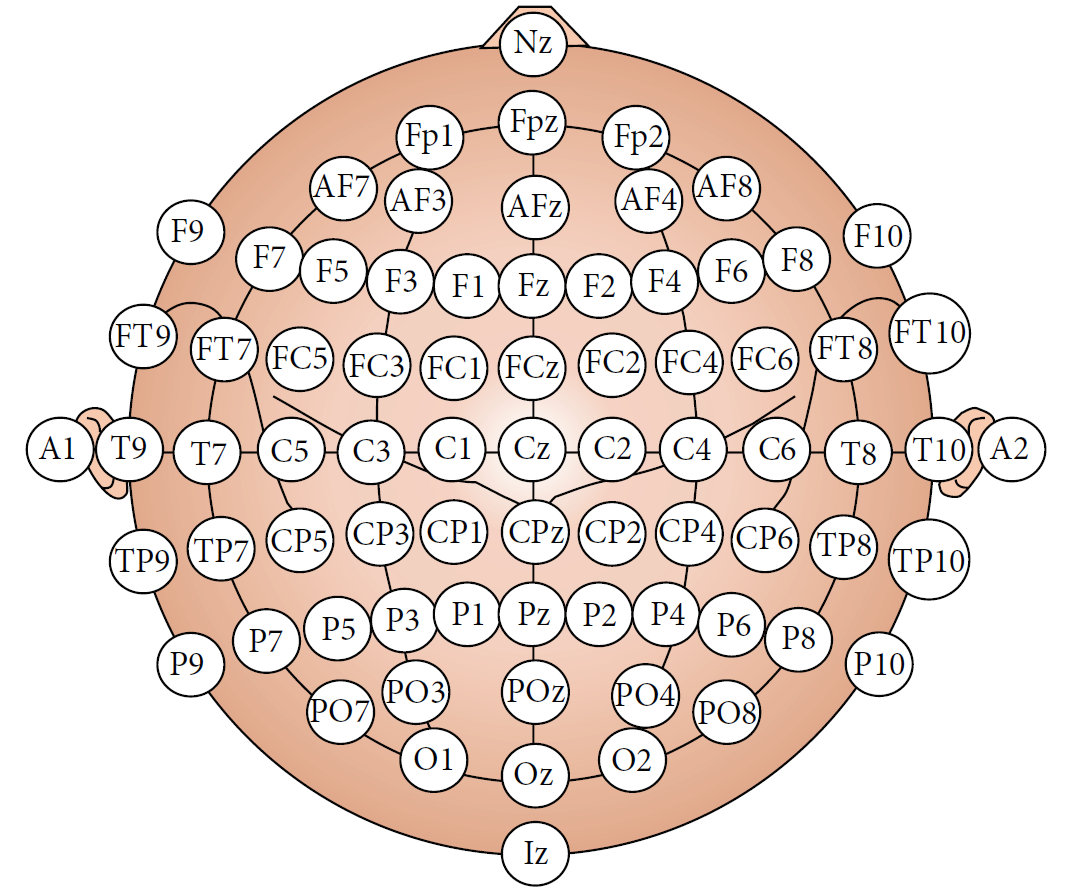
\includegraphics[width=10cm]{Figures/eegcollect.png}
	\caption[Location of the electrodes over the head of the subject]{Location of the electrodes over the head of the subject}
	\label{fig:eegcollect}
\end{figure}

The EEG signals refer to recordings of one minute during a state of no-task with closed eyes, or say "resting state". The data is collected by a helmet on the head. The helmet contains 56 electrodes all over the head, as shown in the \fref{fig:eegcollect}. The sampling frequency is equal to 200 Hz, so each file contains a matrix of 56 x 12000. 

The preprocessing for the data is normalization. I have linearly normalize the sensor values to [0,1] by:
\[ x_{i}' = \frac{x_{i}-x_{min}}{x_{max}-x_{min}} \] 
where $ x_{min} $ and $ x_{max} $ are the minimum and maximum sensor value on the session.

\section{Architecture of Dann EEG}
The principle for our adaption is that we treat session one of each subject EEG data as source domain in the Domain Adaptation, and the session two as the target domain. Once we using the DANN for training, the model will not be able to distinguish which session the input data belongs to, this is to say we can't tell the difference between session one and session two. So after reconstruction, the EEG data from two sessions become indistinguishable.

The base of our DANN is auto-encoder. An autoencoder, autoassociator or Diabolo network\cite{bengio2009learning} is an artificial neural network used for unsupervised learning of efficient codings.\cite{liou2008modeling} The aim of an autoencoder is to learn a representation (encoding) for a set of data, typically for the purpose of dimensionality reduction. Recently, the autoencoder concept has become more widely used for learning generative models of data.\cite{kingma2013auto}

Considering that the input data dimension is 56, so in the input layer and output layer of our Neural Network, the size will be 56. In this internship, which is as a first approach to solve the problem, we use a simple structure with 1 hidden layer like 56 - n -56, where n varies from 1 to 56. 

Above is the base structure of our neural network which is an auto-encoder. Then we need to add the gradient reversal layer which connected to the hidden layer. So the structure is shown in \fref{fig:eegstructure}

\begin{figure}[htbp]
	\centering
	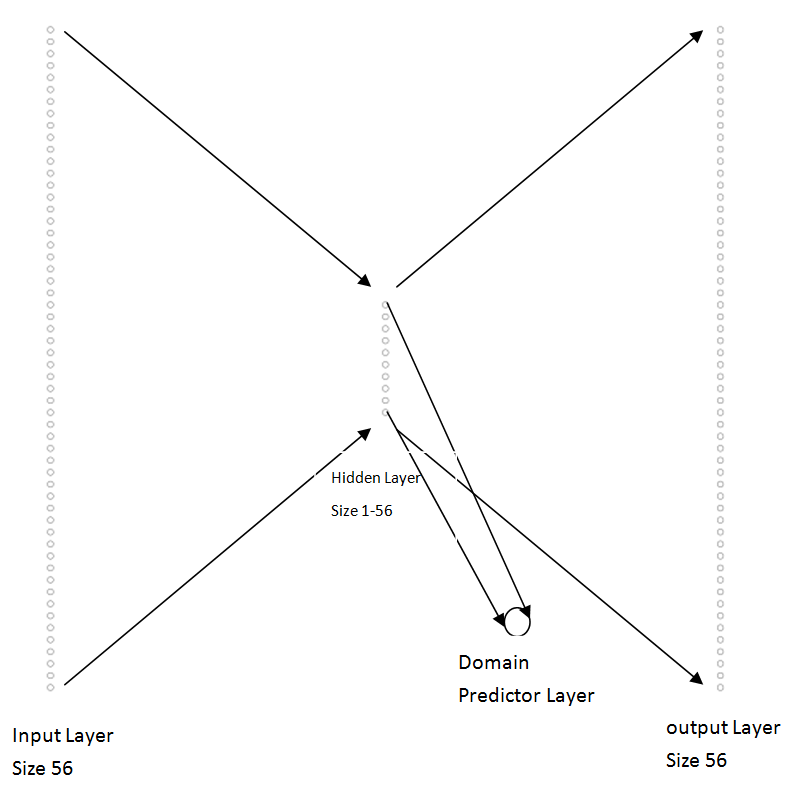
\includegraphics[width=15cm]{Figures/eegstructure.png}
	\caption[Structure of DANN for EEG data]{Structure of DANN for EEG data}
	\label{fig:eegstructure}
\end{figure}


At every neuron, the activation function will using \textbf{Sigmoid}.


\section{Criteria}
For our neural network, there are 2 purposes:
\begin{enumerate}
	\item Minimize the reconstruction error of the EEG data.
	\item Maximize the domain(session) prediction error, so that the sessions cannot be discriminated, even with the best classifier.
\end{enumerate}

Considering the requirements above, two criterion functions will be defined in the program. 

\begin{enumerate}
	\item For the reconstruction loss of EEG, we want to be able to reconstruct the initial EEG data, so we choose the MSE cost function(mean square error) like:
	\[ loss(x, \tilde{x}) = \frac{1}{n} \times \sum_{i=1}^{56}| x_{i}-\tilde{x_{i}}|^2 \]

	\item The second criterion is session-invariant. We will assess this criterion by measuring the BCE(Binary Cross Entropy) criterion of the domain(session) predictor. So the loss function will be:
	\[ loss(o, t) = -\frac{1}{n} \sum(t[i]\times \log o[i]  +  (1-t[i])\times\log (1-o[i]) \]
	where o is original prediction and t is target prediction. This criterion will give the entropy of the error, so when the result have a lot surprise, criterion will be large, otherwise the criterion will be 0.
\end{enumerate}

\section{Framework}
To realize this neural network, I have using the \textbf{Torch} framework. Torch is a scientific computing framework with wide support for machine learning algorithms that puts GPUs first. It is easy to use and efficient, thanks to an easy and fast scripting language, LuaJIT, and an underlying C/CUDA implementation.

In the torch, there's already a \textbf{gradient reversal layer} prepared to use, so we can easy connect the auto-encoder with the gradient reversal layer to build our neural network.

In the program, I have defined three separate neural network, which are:
\begin{enumerate}
	\item \textbf{Encoder}, the structure is 56 - n ($ n \in [1,56] $), this layer is used like feature extractor in the DANN, it also serves as a conpression part.
	\item \textbf{Decoder}, the structure is n - 56 ($ n \in [1,56] $), this layer is used like label predictor in the DANN, it also serves to decode the data to get the initial data.
	\item \textbf{Gradient reversal Layer}, the structure is n - 1 ($ n \in [1,56] $), this layer is used to predict which domain the instance is belonged to. With the help of negative gradient for this layer, we can maximize the error to make the two session indistinguishable. 
\end{enumerate}

Then in the training phase, the EEG data will be used as input data for Encoder, the output of Encoder will then be used as the input data of Decoder and Gradient reversal layer.

Here below is the Lua code used to build our neural network.
\begin{lstlisting}[mathescape]
	//Definition of the encoder
	featExtractor = nn.Sequential()
	featExtractor:add(nn.Linear(nInputEEG,opt.hiddenLayerUnits))
	featExtractor:add(nn.Sigmoid())
	
	//Definition of the decoder
	labelPredictor = nn.Sequential()
	labelPredictor:add(nn.Linear(opt.hiddenLayerUnits,nInputEEG))
	labelPredictor:add(nn.Sigmoid())
	
	//Definition of the domain classifier
	domainClassifier = nn.Sequential()
	domainClassifier:add(nn.GradientReversal(opt.domainLambda))
	domainClassifier:add(nn.Linear(opt.hiddenLayerUnits,1))
	domainClassifier:add(nn.Sigmoid())


\end{lstlisting}